\documentclass[uplatex]{jsarticle}
\usepackage{amsmath}
\usepackage[dvipdfmx]{graphicx}

\setcounter{tocdepth}{3}
\usepackage{float}
\usepackage{moreverb}
\usepackage{lscape}
%\pagestyle{empty}
%\usepackage{wrapfig}
\usepackage{url}
%\usepackage{EasyLayout}

\usepackage{ascmac}
%\usepackage{fancybx}

%\pagestyle{myheadings}



\begin{document}


\title{2分法とニュートン法の収束速度の比較}
\author{25G1051 近藤巧望}
%\date{2015年11月13日}
\maketitle


\section{はじめに}
% この下の行に入力
\subsection{背景}
線形方程式は数学的に扱いやすく,線形に近似できるのであれば線形方程式が有効である.
しかし,自然界での現象は多くが非線形であり,線形方程式では限界があるため,現象の数値解析には非線形方程式を用いた方法が一般的である\cite{ref1}.
つまり,非線形方程式の解を求めることは数値解析において重要な課題である.
また,現象の数値解析において,効率性と確実性は重要な要素であり,
膨大なデータ量を扱う際には計算の効率性が求められ,結果の信頼性を得るためには確実性が求められる\cite{ref2}.
\par
非線形方程式の解を求めるための数値解析方法として2分法とニュートン法があり,
2分法は,中間値の定理という数学的な理論を用いて,区間を2等分しながら解を絞り込む手法であり,
ニュートン法は接線を利用して収束する解を求める手法である.
この二つの数値解析方法は解の収束速度が異なる.
\par
\subsection{目的}
そこで本レポートでは,2分法とニュートン法による解の収束速度を調べることによって,
2分法とニュートン法の特性を比較し,2分法とニュートン法それぞれの適切な活用方法について考えることを目的とする.
\par
\subsection{主張}
非線形方程式の解を求めるために2分法とニュートン法を用いて数値計算を行い,それによって得られたグラフの結果を基に考察する.
グラフでの結果から2分法とニュートン法の収束までの変化傾向や収束速度を比較することにより,双方の特性を明らかにする事ができ,
2分法とニュートン法の適切な活用方法を考察する事ができると考える.



%ニュートン法は明治大学「3.1 ニュートン法」から,2分法はwikiより
\section{手法}
% この下の行に入力
\subsection{方程式の説明}

本レポートでは,(\ref{eq:1})式に示される関数$f(x)$の$f(x)=0$の解を2分法とニュートン法により求める.

\begin{equation}
f(x)=\cos x- x^2\label{eq:1}
\end{equation}


\indent
この方程式は非線形方程式であり,代数的に解くことはできず,グラフや数値計算により解を求める必要がある\cite{ref3}.
なお,本レポートでは,C言語を用いて数値計算を行う.
\indent
また,非線形方程式$f(x)=cos x- x^2$のグラフは図1のとおりである.
\begin{figure}[H]
	\centering
	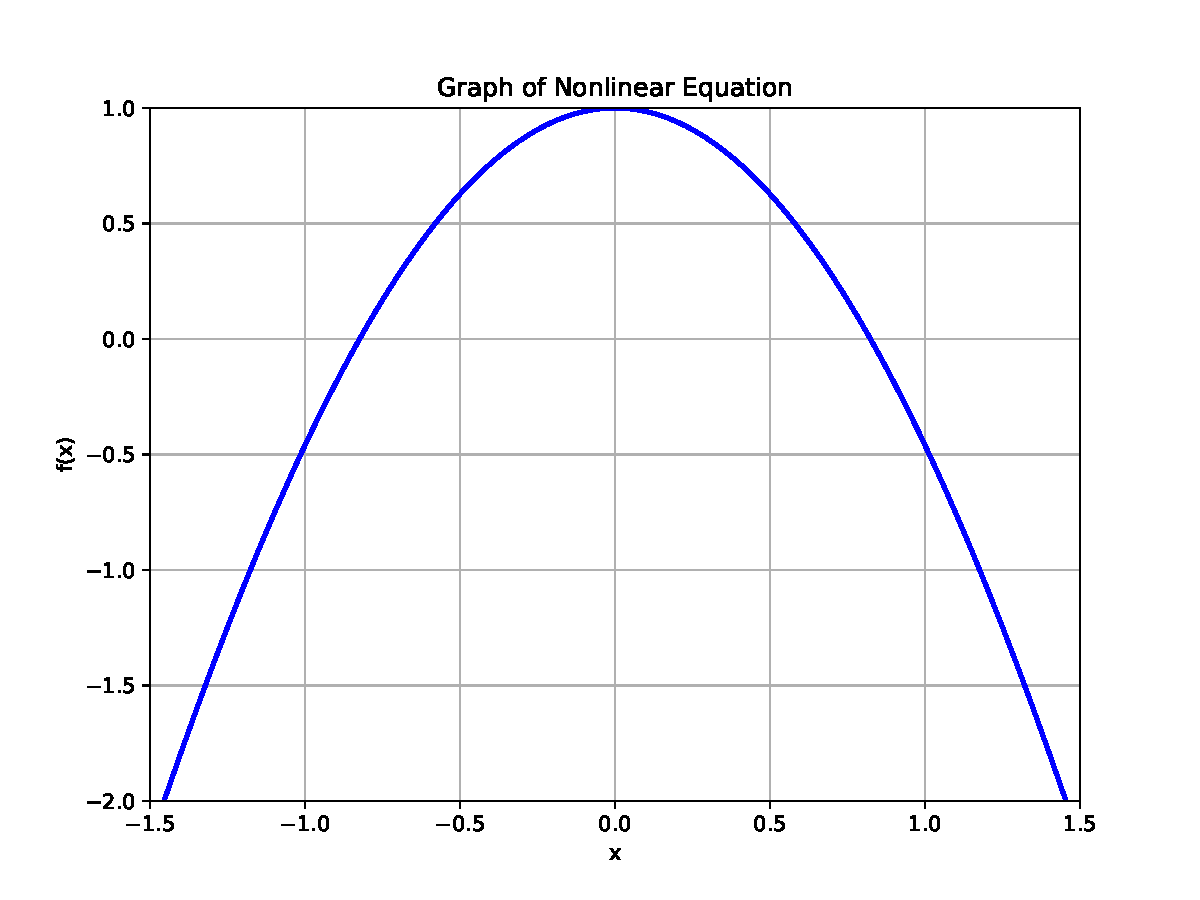
\includegraphics[width=12cm]{./Figs/第6回課題.pdf}
	\caption{非線形方程式$f(x)=cos x- x^2$を表すグラフ.複数の解を持つことがわかる.}
	\label{fig:1}
\end{figure}

\subsection{2分法・ニュートン法の説明}
\indent
2分法とニュートン法について説明する.
\par
まず,2分法の説明のために中間値の定理について説明する.
中間値の定理とは,連続関数$f(x)$が区間$[a,b]$で定義され,$f(a)$と$f(b)$の符号が異なるとき,$f(x)=0$となる点$c$が区間$[a,b]$に存在することを示す定理である.
2分法は,中間値の定理を利用し,解を含む区間の中間点を求める操作を繰り返すことによって方程式を解く方法である.
2分法は,1817年、ベルナルド・ボルツァーノは図形的議論を一切使わず、連続関数が符号変化を起こす区間には必ず実数根が存在することを証明した。
この証明には現代の二分法と同様の区間縮小手法が含まれており、数値解析的ルーツとして位置づけられる.
中間値の定理がボルツァーノによって証明された後に2分法が発展した\cite{ref4}.
使用方法としては,方程式 f(x) = 0 の解を,適当な初期値 a, b から出発して,(\ref{eq:3})の漸化式の極限
で求める方法である\cite{ref5}.
\begin{equation}
x_{n+1} = \frac{a_n + b_n}{2}\label{eq:3}
\end{equation}
また,2分法のアルゴリズムは表\ref{tab:1}のようになる.
\begin{table}[H]
	\centering
	\caption{2分法のアルゴリズム}
	\begin{tabular}{|c|c|}
		\hline
		\textbf{ステップ} & \textbf{説明} \\
		\hline
		1 & $f(x)$を指定し,a, b及び正数εを設定.\\
		& ただし$f(a)f(b)<0$とする.条件が満足されなければa, bを再設定.\\
		\hline
		2 & $c = \frac{a+b}{2}$を計算する. \\
		\hline
		3 & $|c-a|<\epsilon$ならば解を$c$として終了. \\
		\hline
		4 & もし$f(a)f(c)<0$ならば$b=c$として,ステップ2に戻る. \\
		\hline
		5 & そうでなければ$a=c$としてステップ2に戻る. \\
		\hline
	\end{tabular}
	\label{tab:1}
\end{table}
\indent
ニュートン法は,アイザック・ニュートンとジョセフ・ラフソンに由来するとされており,接線を利用して収束する解を求める方法である。
この技術は、17世紀から18世紀の数学者たちが関心を寄せていた三次方程式やそれ以上の高次方程式の解法の研究の中から発展してきた\cite{ref6}.
使用方法としては,方程式 f(x) = 0 の解を,適当な初期値 x0 から出発して,(\ref{eq:4})の漸化式の解が収束するまで反復計算を行う方法である.
\begin{equation}
x_{n+1} = x_n - \frac{f(x_n)}{f'(x_n)}\label{eq:4}
\end{equation}
また,ニュートン法のアルゴリズムは表\ref{tab:2}のようになる.
\begin{table}[H]
	\centering
	\caption{ニュートン法のアルゴリズム}
	\begin{tabular}{|c|c|}
		\hline
		\textbf{ステップ} & \textbf{説明} \\
		\hline
		1 & $f(x)$, $f’(x)$を指定し, $x_0$を設定する.\\
		\hline
		2 & $n=0,1,2,…$に対して,(\ref{eq:4})の反復演算を$x_n$が収束するまで繰り返す. \\
		\hline
		3 & 収束すれば反復終了. \\
		\hline
	\end{tabular}
	\label{tab:2}
\end{table}

\subsection{プログラムの仕様}
\indent
ここからは,本レポートで使用する2分法とニュートン法のC言語でのプログラムについて説明する.
\par

まずは2分法のプログラムについて説明する.
この関数は2分法を用いて方程式$\cos x - x^2 = 0$の近似解を求める.
引数として区間の下限$a$,上限$b$,および許容誤差$tol$を受け取り,
計算が成功した場合は近似解を,失敗した場合は$-1$を返り値として出力する.
本プログラムでは,$a=0.0$,$b=1.0$,$tol=0.00001$と設定している.
\par

次にニュートン法のプログラムについて説明する.
この関数はニュートン法を用いて方程式$\cos x - x^2 = 0$の近似解を求める.
引数として初期値$x_0$,許容誤差$tol$,最大反復回数$max\_iter$を受け取り,
計算が成功した場合は近似解を,失敗した場合は$-1$を返り値として出力する.
本プログラムでは,$x_0=0.5$,$tol=0.00001$,$max\_iter=1000$と設定している.


\subsection{評価指標}
\indent
本レポートでは,2分法とニュートン法の収束までの反復回数を,2分法とニュートン法の収束速度として評価する.
つまり,収束までに要した反復回数が少ないほど,収束速度が速いとみなす.
この評価指標は,数値解析における一般的な収束性評価法であり\cite{ref7},実用性の観点から妥当である.
なぜなら,解が収束するまでの反復回数が少ないほど,必要な計算リソースが少なくて済むためである.
さらに,導き出した収束速度を比較することにより,2分法とニュートン法の特性を考察する.

\section{結果}
\begin{figure}[H]
	\centering
	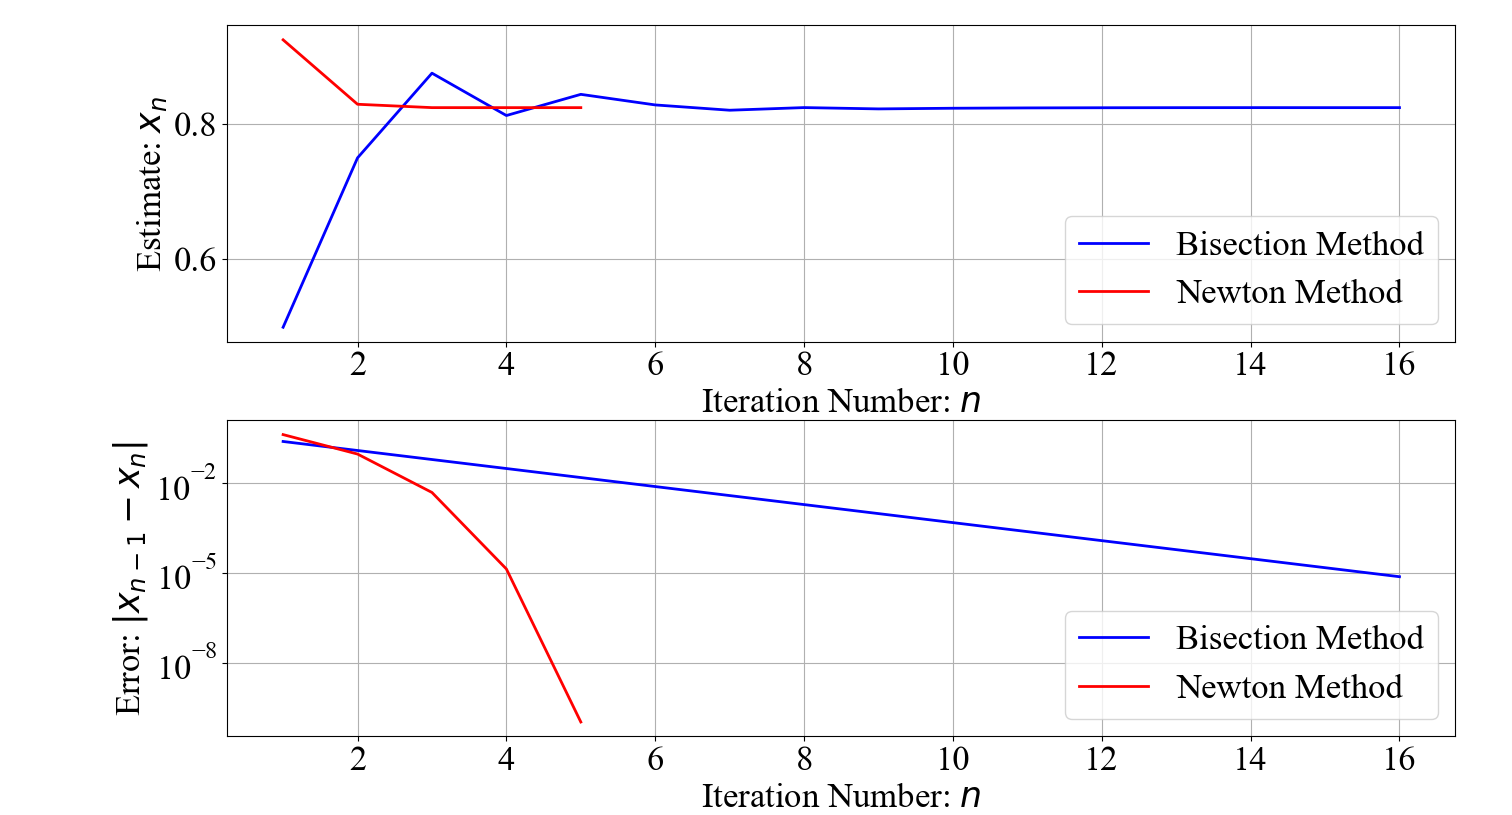
\includegraphics[width=12cm]{./Figs/Figure_1.png}
	\caption{2分法とニュートン法における推定解の反復回数$n$に対する依存性
	(上図)、それぞれの場合における誤差$|x_n−x_{n+1}|$の反復回数に対する依存性
	(下図)。2分法とニュートン法の両者とも、$x_n → 0.824$付近に収束し、
	ニュートン法の方が収束に要する反復回数が少ない。}
    \label{fig:2}
\end{figure}

\indent
2分法とニュートン法における推定解の反復回数$n$に対する依存性と
それぞれの場合における誤差$|x_n−x_{n+1}|$の反復回数に対する依存性を図\ref{fig:2}に示す.
結果として,2分法とニュートン法の両方とも$x_n→0.824$付近に収束した.
\par
また,図\ref{fig:2}からわかるように,2分法に比べてニュートン法の方が収束までに要する反復回数が少ないことがわかる.
具体的には,2分法は16回の反復でも収束しなかったのに対し,ニュートン法は約5回の反復で収束した.
また,ニュートン法の誤差は2分法に比べて急激に減少しており,2分法では,解の推定値が真の解に近づくにつれて誤差が徐々に減少していく様子が見られる.
\par

\section{おわりに}
\indent
本レポートでは,2分法とニュートン法の活用方法について考えることを目的とし,
2分法とニュートン法を用いて非線形方程式の解を求め,2分法とニュートン法による
解の収束速度を比較した.
その結果,二分法は少しずつ収束したのに対し,
ニュートン法は少ない反復回数で収束したことがわかった.
\par
ここからは,2分法とニュートン法の特徴について考察する.
結果から2分法とニュートン法を比較すると,収束に要する反復回数がより少なく済んだニュートン法は,2分法よりも収束速度が速いと言える.
つまり,ニュートン法は効率性の観点からは優れていると考えられる.
しかし2分法は,ニュートン法と違い初期値を選ぶ必要がなく,単純な方法であるため,安定した解を求めることができるという利点がある.
そのため,2分法よりニュートン法の収束速度が速いとはいえ,すべての点においてニュートン法が優れているとは言えず,
2分法とニュートン法は状況によって使い分ける必要があると考えられる.
\par
二つの数値解析方法にそれぞれの利点がある一方で,それぞれ注意点もある.
2分法は,収束速度が遅いため,計算に時間がかかることがある.これは,解を求めるために多くの反復が必要になるためである.
図\ref{fig:2}からもわかるように,2分法は収束までに多くの反復回数を要している.
ニュートン法では,初期値が解から離れていると収束しない場合があるため,注意が必要である.
そのため,初期値を適切に選ぶ必要がある.
また,ニュートン法は,関数の導関数を必要とするため,関数の性質によっては導関数が計算できない場合もある.
そのため,ニュートン法を適用する際には,関数の導関数が存在するかどうかを確認する必要がある.
今回の場合は,初期値が$x_0=0.5$であり,関数$f(x)=\cos x - x^2$の導関数$f'(x)=-\sin x - 2x$は計算可能であるため,
ニュートン法を適用することができた.

\par
以上のように,2分法とニュートン法はそれぞれの特性を持っており,適切な方法を選択することが重要である.
具体的には,確実性が求められる場合には,安定して解を求めることができる2分法を活用し,
効率性を重視する場合には,収束速度が速いニュートン法を活用することが妥当であると考えられる.

\begin{thebibliography}{9}
\bibitem{ref1}William R. Perkins,「Nonlinear Phenomen」,

\url{https://www.sciencedirect.com/topics/engineering/nonlinear-phenomenon}
\bibitem{ref2} Mathematics Institute of Computational Science and Engineering, 「MATHICSE Technical Report
Nr. 13.2013
April 2013 (NEW 10.2013)」,

\url{https://www.epfl.ch/labs/mathicse/wp-content/uploads/2018/10/13.2013_NEW_PC-AQ.pdf}
\bibitem{ref3} Ghazala Gulshan, Hüseyin Budak, Rashida Hussain and Asad Sadiq
「Generalization of the bisection method and its applications in nonlinear equations」,

\url{https://advancesincontinuousanddiscretemodels.springeropen.com/articles/10.1186/s13662-023-03765-5}
\bibitem{ref4} Wojciech Kryszewski,「The legacy of Bolzano-Miranda-Poincaré intermediate value theorem」,

\url{https://www.aimsciences.org/article/doi/10.3934/mcrf.2024048}
\bibitem{ref5} 早稲田大学「非線形方程式の解法 (1)」,

\url{https://yuuka.w.waseda.jp/cpro2/Cpro2_10th.pdf}
\bibitem{ref6} Geospatial Science,「NEWTON-RAPHSON ITERATION」,

\url{https://www.mygeodesy.id.au/documents/Newton-Raphson%20Iteration.pdf}
\bibitem{ref7} 森正武「数値解析」,共立出版,1995年
\end{thebibliography}

\end{document}



























